\documentclass[conference]{IEEEtran}
% Some Computer Society conferences also require the compsoc mode option,
% but others use the standard conference format.
%
% If IEEEtran.cls has not been installed into the LaTeX system files,
% manually specify the path to it like:
% \documentclass[conference]{../sty/IEEEtran}

\usepackage[utf8]{inputenc}
% Especifica la codificación de caracteres de los documentos.

%\usepackage[spanish]{babel}
% Indica que el documento se escribirá en español.
% Traduce algunos comandos que no poseen versión en español
%\def\IEEEkeywordsname{Palabras Claves}
%\def\IEEEproofname{Demostración}

% Some very useful LaTeX packages include:
% (uncomment the ones you want to load)

% *** MISC UTILITY PACKAGES ***
%
%\usepackage{ifpdf}
% Heiko Oberdiek's ifpdf.sty is very useful if you need conditional
% compilation based on whether the output is pdf or dvi.
% usage:
% \ifpdf
%   % pdf code
% \else
%   % dvi code
% \fi
% The latest version of ifpdf.sty can be obtained from:
% http://www.ctan.org/pkg/ifpdf
% Also, note that IEEEtran.cls V1.7 and later provides a builtin
% \ifCLASSINFOpdf conditional that works the same way.
% When switching from latex to pdflatex and vice-versa, the compiler may
% have to be run twice to clear warning/error messages.

% *** CITATION PACKAGES ***
%
%\usepackage{cite}
% cite.sty was written by Donald Arseneau
% V1.6 and later of IEEEtran pre-defines the format of the cite.sty package
% \cite{} output to follow that of the IEEE. Loading the cite package will
% result in citation numbers being automatically sorted and properly
% "compressed/ranged". e.g., [1], [9], [2], [7], [5], [6] without using
% cite.sty will become [1], [2], [5]--[7], [9] using cite.sty. cite.sty's
% \cite will automatically add leading space, if needed. Use cite.sty's
% noadjust option (cite.sty V3.8 and later) if you want to turn this off
% such as if a citation ever needs to be enclosed in parenthesis.
% cite.sty is already installed on most LaTeX systems. Be sure and use
% version 5.0 (2009-03-20) and later if using hyperref.sty.
% The latest version can be obtained at:
% http://www.ctan.org/pkg/cite
% The documentation is contained in the cite.sty file itself.

% *** GRAPHICS RELATED PACKAGES ***
%
\ifCLASSINFOpdf
  \usepackage[pdftex]{graphicx}
  % declare the path(s) where your graphic files are
  % \graphicspath{{../pdf/}{../jpeg/}}
  % and their extensions so you won't have to specify these with
  % every instance of \includegraphics
  % \DeclareGraphicsExtensions{.pdf,.jpeg,.png}
\else
  % or other class option (dvipsone, dvipdf, if not using dvips). graphicx
  % will default to the driver specified in the system graphics.cfg if no
  % driver is specified.
  \usepackage[dvips]{graphicx}
  % declare the path(s) where your graphic files are
  % \graphicspath{{../eps/}}
  % and their extensions so you won't have to specify these with
  % every instance of \includegraphics
  % \DeclareGraphicsExtensions{.eps}
\fi
% graphicx was written by David Carlisle and Sebastian Rahtz. It is
% required if you want graphics, photos, etc. graphicx.sty is already
% installed on most LaTeX systems. The latest version and documentation
% can be obtained at: 
% http://www.ctan.org/pkg/graphicx
% Another good source of documentation is "Using Imported Graphics in
% LaTeX2e" by Keith Reckdahl which can be found at:
% http://www.ctan.org/pkg/epslatex
%
% latex, and pdflatex in dvi mode, support graphics in encapsulated
% postscript (.eps) format. pdflatex in pdf mode supports graphics
% in .pdf, .jpeg, .png and .mps (metapost) formats. Users should ensure
% that all non-photo figures use a vector format (.eps, .pdf, .mps) and
% not a bitmapped formats (.jpeg, .png). The IEEE frowns on bitmapped formats
% which can result in "jaggedy"/blurry rendering of lines and letters as
% well as large increases in file sizes.
%
% You can find documentation about the pdfTeX application at:
% http://www.tug.org/applications/pdftex

% *** MATH PACKAGES ***
%
%\usepackage{amsmath}
% A popular package from the American Mathematical Society that provides
% many useful and powerful commands for dealing with mathematics.
%
% Note that the amsmath package sets \interdisplaylinepenalty to 10000
% thus preventing page breaks from occurring within multiline equations. Use:
%\interdisplaylinepenalty=2500
% after loading amsmath to restore such page breaks as IEEEtran.cls normally
% does. amsmath.sty is already installed on most LaTeX systems. The latest
% version and documentation can be obtained at:
% http://www.ctan.org/pkg/amsmath

% *** SPECIALIZED LIST PACKAGES ***
%
%\usepackage{algorithmic}
% algorithmic.sty was written by Peter Williams and Rogerio Brito.
% This package provides an algorithmic environment fo describing algorithms.
% You can use the algorithmic environment in-text or within a figure
% environment to provide for a floating algorithm. Do NOT use the algorithm
% floating environment provided by algorithm.sty (by the same authors) or
% algorithm2e.sty (by Christophe Fiorio) as the IEEE does not use dedicated
% algorithm float types and packages that provide these will not provide
% correct IEEE style captions. The latest version and documentation of
% algorithmic.sty can be obtained at:
% http://www.ctan.org/pkg/algorithms
% Also of interest may be the (relatively newer and more customizable)
% algorithmicx.sty package by Szasz Janos:
% http://www.ctan.org/pkg/algorithmicx

% *** ALIGNMENT PACKAGES ***
%
%\usepackage{array}
% Frank Mittelbach's and David Carlisle's array.sty patches and improves
% the standard LaTeX2e array and tabular environments to provide better
% appearance and additional user controls. As the default LaTeX2e table
% generation code is lacking to the point of almost being broken with
% respect to the quality of the end results, all users are strongly
% advised to use an enhanced (at the very least that provided by array.sty)
% set of table tools. array.sty is already installed on most systems. The
% latest version and documentation can be obtained at:
% http://www.ctan.org/pkg/array

% IEEEtran contains the IEEEeqnarray family of commands that can be used to
% generate multiline equations as well as matrices, tables, etc., of high
% quality.

% *** SUBFIGURE PACKAGES ***
%\ifCLASSOPTIONcompsoc
%  \usepackage[caption=false,font=normalsize,labelfont=sf,textfont=sf]{subfig}
%\else
%  \usepackage[caption=false,font=footnotesize]{subfig}
%\fi
% subfig.sty, written by Steven Douglas Cochran, is the modern replacement
% for subfigure.sty, the latter of which is no longer maintained and is
% incompatible with some LaTeX packages including fixltx2e. However,
% subfig.sty requires and automatically loads Axel Sommerfeldt's caption.sty
% which will override IEEEtran.cls' handling of captions and this will result
% in non-IEEE style figure/table captions. To prevent this problem, be sure
% and invoke subfig.sty's "caption=false" package option (available since
% subfig.sty version 1.3, 2005/06/28) as this is will preserve IEEEtran.cls
% handling of captions.
% Note that the Computer Society format requires a larger sans serif font
% than the serif footnote size font used in traditional IEEE formatting
% and thus the need to invoke different subfig.sty package options depending
% on whether compsoc mode has been enabled.
%
% The latest version and documentation of subfig.sty can be obtained at:
% http://www.ctan.org/pkg/subfig

% *** FLOAT PACKAGES ***
%
%\usepackage{fixltx2e}
% fixltx2e, the successor to the earlier fix2col.sty, was written by
% Frank Mittelbach and David Carlisle. This package corrects a few problems
% in the LaTeX2e kernel, the most notable of which is that in current
% LaTeX2e releases, the ordering of single and double column floats is not
% guaranteed to be preserved. Thus, an unpatched LaTeX2e can allow a
% single column figure to be placed prior to an earlier double column
% figure.
% Be aware that LaTeX2e kernels dated 2015 and later have fixltx2e.sty's
% corrections already built into the system in which case a warning will
% be issued if an attempt is made to load fixltx2e.sty as it is no longer
% needed.
% The latest version and documentation can be found at:
% http://www.ctan.org/pkg/fixltx2e

\usepackage{stfloats}
% stfloats.sty was written by Sigitas Tolusis. This package gives LaTeX2e
% the ability to do double column floats at the bottom of the page as well
% as the top. (e.g., "\begin{figure*}[!b]" is not normally possible in
% LaTeX2e). It also provides a command:
%\fnbelowfloat
% to enable the placement of footnotes below bottom floats (the standard
% LaTeX2e kernel puts them above bottom floats). This is an invasive package
% which rewrites many portions of the LaTeX2e float routines. It may not work
% with other packages that modify the LaTeX2e float routines. The latest
% version and documentation can be obtained at:
% http://www.ctan.org/pkg/stfloats
% Do not use the stfloats baselinefloat ability as the IEEE does not allow
% \baselineskip to stretch. Authors submitting work to the IEEE should note
% that the IEEE rarely uses double column equations and that authors should try
% to avoid such use. Do not be tempted to use the cuted.sty or midfloat.sty
% packages (also by Sigitas Tolusis) as the IEEE does not format its papers in
% such ways.
% Do not attempt to use stfloats with fixltx2e as they are incompatible.
% Instead, use Morten Hogholm'a dblfloatfix which combines the features
% of both fixltx2e and stfloats:
%
% \usepackage{dblfloatfix}
% The latest version can be found at:
% http://www.ctan.org/pkg/dblfloatfix

% *** PDF, URL AND HYPERLINK PACKAGES ***
%
%\usepackage{url}
% url.sty was written by Donald Arseneau. It provides better support for
% handling and breaking URLs. url.sty is already installed on most LaTeX
% systems. The latest version and documentation can be obtained at:
% http://www.ctan.org/pkg/url
% Basically, \url{my_url_here}.


% *** Do not adjust lengths that control margins, column widths, etc. ***
% *** Do not use packages that alter fonts (such as pslatex).         ***
% There should be no need to do such things with IEEEtran.cls V1.6 and later.
% (Unless specifically asked to do so by the journal or conference you plan
% to submit to, of course. )


% correct bad hyphenation here
%\hyphenation{op-tical net-works semi-conduc-tor}


\begin{document}
%
% paper title
% Titles are generally capitalized except for words such as a, an, and, as,
% at, but, by, for, in, nor, of, on, or, the, to and up, which are usually
% not capitalized unless they are the first or last word of the title.
% Linebreaks \\ can be used within to get better formatting as desired.
% Do not put math or special symbols in the title.
\title{Drone’s Shared Knowledge\\for Product Delivery Service}


% author names and affiliations
% use a multiple column layout for up to three different
% affiliations
%\author{\IEEEauthorblockN{Marco Lotto}
%\IEEEauthorblockA{Facultad de Ingeniería\\
%Universidad de Buenos Aires\\
%Georgia Institute of Technology\\
%Atlanta, Georgia 30332--0250\\
%Email: }
%\and
%\IEEEauthorblockN{Ezequiel Pérez Dittler}
%\IEEEauthorblockA{Facultad de Ingeniería\\
%Universidad de Buenos Aires\\
%Springfield, USA\\
%Email: ezperez@fi.uba.ar}
%\and
%\IEEEauthorblockN{Tomás Reale}
%\IEEEauthorblockA{Facultad de Ingeniería\\
%Universidad de Buenos Aires\\
%San Francisco, California 96678--2391\\
%Telephone: (800) 555--1212\\
%Fax: (888) 555--1212
%Email: }
%\and
%\IEEEauthorblockN{Migue Torres}
%\IEEEauthorblockA{Facultad de Ingeniería\\
%Universidad de Buenos Aires\\
%Email: }
%}

% conference papers do not typically use \thanks and this command
% is locked out in conference mode. If really needed, such as for
% the acknowledgment of grants, issue a \IEEEoverridecommandlockouts
% after \documentclass

% for over three affiliations, or if they all won't fit within the width
% of the page, use this alternative format:
% 
\author{
\IEEEauthorblockN{
Marco Lotto\IEEEauthorrefmark{1},
Ezequiel Pérez Dittler\IEEEauthorrefmark{1},
Tomás Reale\IEEEauthorrefmark{1} y
Miguel Torres\IEEEauthorrefmark{1}}
\IEEEauthorblockA{
\IEEEauthorrefmark{1}Facultad de Ingeniería,
Universidad de Buenos Aires, Argentina}}


% use for special paper notices
%\IEEEspecialpapernotice{(Invited Paper)}


% make the title area
\maketitle

% As a general rule, do not put math, special symbols or citations
% in the abstract
\begin{abstract}
The technological progress of Unmanned Aerial Vehicles (UAV) and the rise of drones on a massive scale suggest that the time has come to start solving everyday problems (like product delivery) with them.
A common property to most UAVs is that they are either monitored, or have had their routes pre-defined by humans
A delivery drone in a urban environment has limited aerial space, either by buildings, weather conditions, grown trees, scaffolding,etc.
This situation makes it necessary for the drones to have their routes redefined.
Because of this, operating multiple drones simultaneously can become way too expensive and even unmanageable.
Our proposal is to develop an AI for the drones that will allow them to calculate and manage their own routes, taking inputs from the world around them and sharing that knowledge among them in order to improve the overall knowledge of the available aerial space.
\end{abstract}

% keywords

\begin{IEEEkeywords}
Unmanned Aerial Vehicles, UAV, drone, delivery, IA, shared knowledge.
\end{IEEEkeywords}


% For peer review papers, you can put extra information on the cover
% page as needed:
% \ifCLASSOPTIONpeerreview
% \begin{center} \bfseries EDICS Category: 3-BBND \end{center}
% \fi
%
% For peerreview papers, this IEEEtran command inserts a page break and
% creates the second title. It will be ignored for other modes.
\IEEEpeerreviewmaketitle


\section{Introduction}
%\hfill Mayo 2016


The origin of drones can be traced back to middle of the 19th century when the Austrian military attacked the enemy Italian city of Venice using balloons laden with explosives, but being entirely at the whim of the wind, a dangerously unpredictable flight-path saw many explode over Austrian territory. In 1898, inventor Nikola Tesla displayed a small unmanned boat that appears to change direction on verbal command. He used RF to change the course of the boat. In 1915, he gave a dissertation on using armed pilotless aircraft capable of defending US.\\

Drones similar to the one’s used today started showing during the WW II.
In \textbf{2005}, drones started entering the \textbf{consumer market space} and the FAA came up with a memorandum of interim policy, which approved the use of domestic drones and helped drone operators fly at the same standard as pilots.
In the following years the FAA restricted that policy and made it a requirement to have a certificate of authorization by FAA to fly drones. This applied to companies, government 
agencies and universities. This slowed down the commercial applications as very few
authorizations were issued. In 2012, Congress enacted FMRA (FAA Modernization and Reform Act), which requires FAA to devise a plan to accelerate and successfully integrate drone usage in the airspace by Fall 2015.\\

\textbf{One of the most widely talked about commercial drones is for freight transport or package deliveries}. \textbf{Amazon} made a big splash when they announced Amazon Prime Air in December 2013 with the stated goal of reducing shipment times to 30 minutes from nearby distribution centers. \textbf{DHL} initiated a pilot program in Sept 2014 to perform parcel deliveries in Germany to reach remote locations near the North Sea. \textbf{Google's} ``Project Wing'' has been testing delivery drones in Australia. \textbf{UPS} is also researching delivery drones, and according to articles, they are considering using drones to move packages between distribution centers and airports to distribution center.\\

Although, drone delivery technology is being developed by a few companies, we will focus in one in particular: \textbf{Amazon}.\\


% An example of a floating figure using the graphicx package.
% Note that \label must occur AFTER (or within) \caption.
% For figures, \caption should occur after the \includegraphics.
% Note that IEEEtran v1.7 and later has special internal code that
% is designed to preserve the operation of \label within \caption
% even when the captionsoff option is in effect. However, because
% of issues like this, it may be the safest practice to put all your
% \label just after \caption rather than within \caption{}.
%
% Reminder: the "draftcls" or "draftclsnofoot", not "draft", class
% option should be used if it is desired that the figures are to be
% displayed while in draft mode.
%
%\begin{figure}[!t]
%\centering
%\includegraphics[width=2.5in]{myfigure}
% where an .eps filename suffix will be assumed under latex, 
% and a .pdf suffix will be assumed for pdflatex; or what has been declared
% via \DeclareGraphicsExtensions.
%\caption{Simulation results for the network.}
%\label{fig_sim}
%\end{figure}

% Note that the IEEE typically puts floats only at the top, even when this
% results in a large percentage of a column being occupied by floats.


% An example of a double column floating figure using two subfigures.
% (The subfig.sty package must be loaded for this to work.)
% The subfigure \label commands are set within each subfloat command,
% and the \label for the overall figure must come after \caption.
% \hfil is used as a separator to get equal spacing.
% Watch out that the combined width of all the subfigures on a 
% line do not exceed the text width or a line break will occur.
%
%\begin{figure*}[!t]
%\centering
%\subfloat[Case I]{\includegraphics[width=2.5in]{box}%
%\label{fig_first_case}}
%\hfil
%\subfloat[Case II]{\includegraphics[width=2.5in]{box}%
%\label{fig_second_case}}
%\caption{Simulation results for the network.}
%\label{fig_sim}
%\end{figure*}
%
% Note that often IEEE papers with subfigures do not employ subfigure
% captions (using the optional argument to \subfloat[]), but instead will
% reference/describe all of them (a), (b), etc., within the main caption.
% Be aware that for subfig.sty to generate the (a), (b), etc., subfigure
% labels, the optional argument to \subfloat must be present. If a
% subcaption is not desired, just leave its contents blank,
% e.g., \subfloat[].


% An example of a floating table. Note that, for IEEE style tables, the
% \caption command should come BEFORE the table and, given that table
% captions serve much like titles, are usually capitalized except for words
% such as a, an, and, as, at, but, by, for, in, nor, of, on, or, the, to
% and up, which are usually not capitalized unless they are the first or
% last word of the caption. Table text will default to \footnotesize as
% the IEEE normally uses this smaller font for tables.
% The \label must come after \caption as always.
%
%\begin{table}[!t]
%% increase table row spacing, adjust to taste
%\renewcommand{\arraystretch}{1.3}
% if using array.sty, it might be a good idea to tweak the value of
% \extrarowheight as needed to properly center the text within the cells
%\caption{An Example of a Table}
%\label{table_example}
%\centering
%% Some packages, such as MDW tools, offer better commands for making tables
%% than the plain LaTeX2e tabular which is used here.
%\begin{tabular}{|c||c|}
%\hline
%One & Two\\
%\hline
%Three & Four\\
%\hline
%\end{tabular}
%\end{table}


% Note that the IEEE does not put floats in the very first column
% - or typically anywhere on the first page for that matter. Also,
% in-text middle ("here") positioning is typically not used, but it
% is allowed and encouraged for Computer Society conferences (but
% not Computer Society journals). Most IEEE journals/conferences use
% top floats exclusively. 
% Note that, LaTeX2e, unlike IEEE journals/conferences, places
% footnotes above bottom floats. This can be corrected via the
% \fnbelowfloat command of the stfloats package.

\begin{figure*}[!t]
\centering
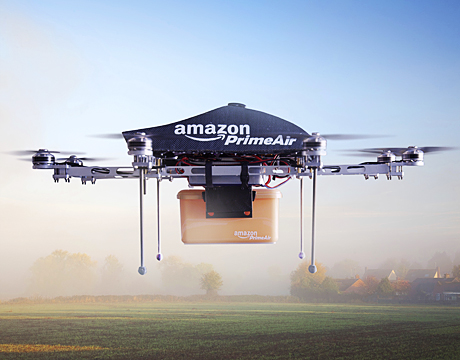
\includegraphics[width=0.5\textwidth]{Developing_Delivery_Drones_hero}
\caption{Amazon Prime Drone}
\label{fig_amazon_prime_drone}
\end{figure*}

\section{State of the art}

\textbf{Amazon} is the pioneer in drone delivery technologies, and security is one major issue. A drone falling from the sky is actually a really serious problem for people's safety and measures have to be taken. It's not the same if a drone flies in a high density area like a city or if a drone flies in a country area. 
They will also need to minimize interaction with lesser-equipped small unmanned aerial vehicles, as well as the occasional manned aircraft flying at low altitude. To ensure the safety and integrity of the overall system, it is paramount that all UAS operators understand where they can and cannot safely operate.\\

Aviation authorities, manufacturers and operators around the world have created high standards for equipment, operations, reliability, and safety. In order to maintain and enhance the level of safety achieved in aviation today for sUAS, aviation authorities should adopt performance-based equipage and operating standards.\\

It is with this in mind that \textbf{Amazon} envisions four separate sUAS equipage classes: \textbf{Basic, Good, Better, and Best}, as we see in \textit{``Determining Safe Access with a Best-Equipped, Best-Served Model for Small Unmanned Aircraft Systems''}. These classes optimize for safe and efficient airspace operations by creating categories of access based on capability. For example, a vehicle with an equipage classification of ‘Good’ does not meet the vehicle capability requirements, such as automated collaborative deconfliction and non-collaborative SAA, that are needed to perform a complex mission in an urban environment. On the other end of the spectrum, operators requesting access to execute missions with high complexity must equip in the `Best' class and possess five equipage elements: (1) geospatial data for safe separation from known hazards, (2) online flight planning and management, (3) reliable Internet connection, (4) collaborative V2V SAA, and (5) non-collaborative sensor-based SAA. It is Amazon's position that these five `Best' equipage elements are essential for safe, highly-automated operations.\\

Of course, this classification is not enough. Another thing to keep in mind is airspace division.

\begin{figure*}[!t]
\centering
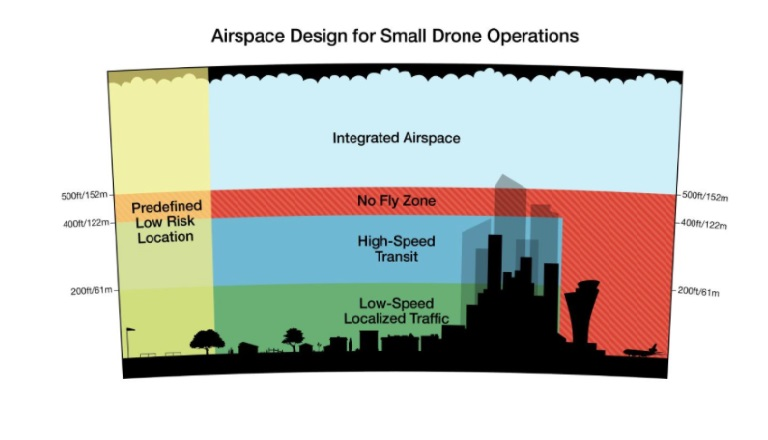
\includegraphics[width=0.85\textwidth]{airspace-design-small-drone-operations}
\caption{Airspace Drone Operations}
\label{fig_airspace_drone_operations}
\end{figure*}

The majority of airspace integration efforts over the past decade have focused on integrating medium or large unmanned aircraft systems into non-segregated civil airspace, i.e. airspace above 500 feet where most civil and military aviation activities occur. However, given the rapidly growing small unmanned aircraft industry, Amazon believes the safest and most efficient environment for sUAS operations—from basic recreational users to sophisticated BLOS fleets—is in segregated civil airspace1 below 500 feet ". Segregating the airspace will buffer sUAS operations from current aviation operations. It will also buffer lesser-equipped vehicles from highly-equipped vehicles able to safely perform BLOS missions.\\

In the proposed model (``Revising the Airspace Model for the Safe Integration of Small Unmanned Aircraft Systems'') below 200 feet, or the `Low-Speed Localized Traffic' area, will be reserved for terminal non-transit operations such as surveying, videography and inspection, and operations for lesser-equipped vehicles, e.g. ones without sophisticated sense-and-avoid (SAA) technology. Those lesser-equipped vehicles will not have access to certain airspace in this zone, such as over heavily-populated areas.
A `High-Speed Transit' space, between 200 and 400 feet, will be designated for well-equipped vehicles as determined by the relevant performance standards and rules.
The airspace between 400 and 500 feet will serve as a permanent `No Fly Zone' in which sUAS operators will not be permitted to fly, except in emergencies.
Finally, this airspace model will also encompass `Predefined Low Risk Locations'. Altitude and equipage restrictions in these locations will be established in advance by aviation authorities. These Predefined Low Risk Locations will include areas like designated Academy of Model Aeronautics airfields, where members will meet pre-established parameters for altitude and equipage.
\textbf{Amazon} believes this segregated airspace model will enable safer overall operations by providing a framework where airspace access is tied to vehicle capability, and by buffering sUAS operations from current aviation operations.\\

\textbf{Other aspect to keep in mind is finding the best paths and drone's battery life}. As a drone's movement is not limited to existing transportation network, path planning needs to be conducted in continuous space with \textbf{taking into account obstacles for flight}. However, due to limited flight range of battery-powered drones, \textbf{multiple recharging stations are required to complete delivery without running out of the power in large urban area}. As we see in \textit{``Deviation flow refueling location model for continuous space: commercial drone delivery system for urban area''},  it is possible to create a coverage model that can optimize location of \textbf{recharging stations} for delivery drones, as well as ensure construction of a feasible delivery network that connects the stations and covered demands based on continuous space shortest paths. A heuristic solution technique is utilized for the optimization of station location. Application results show the effectiveness of this model for construction of drone delivery network that covers large urban area.\\



\section{Shared knowledge}

As we said, our proposal is to develop an AI for the drones that will allow them to calculate and manage their own routes, taking inputs from the world around them and sharing that knowledge among them in order to improve the overall knowledge of the available aerial space.
\textbf{Shared knowledge is the ability to learn information known by other drones and devices connected to the network.} 
For example, if a drone is in an area with high drone density, he may inform to other drones to avoid that area to reduce collision risk. A drone can tell another one to carry packages for him if they go to the same destination.
Drone to drone communication is just one of many, as it can be extended to all kind of devices. For example, a \textbf{weather channel} on the internet can inform drones to avoid certain areas due to bad weather conditions. This is only one example of an online service to assist drones, but it can be extended to a lot of different types of them. 
On the other hand drones can also provide data to users and services, for example \textbf{timing in package distribution, real time street information via photographies}.\\

Physical devices can also communicate with drones. For instance, in the case of \textbf{battery replacement and charging}. As we all know, drones need to be charged regularly. But if drones share info about their battery life, plus the model we saw early in the state of the art section, they can share their payload, accordingly to their size, type of drone and weight, drones that are running low on battery can just stop and reload while other take their package and send them to the specified destination.\\

Other crucial information is the position and trajectory of nearby drones for \textbf{collision detection and avoidance}. Finding optimal paths will not only prevent accidents, but also will reduce delivery times and save fuel.\\


\section{Conclusion}

Drone are here to stay. They are not only the future, but the present as well. Governments of the world should regulate accordingly, not prohibit, their use.
Drones will help the economy, increase competition, increase customer satisfaction,and allow e-commerce to flourish even more.\\

Communication is the key to success in every organization and in every team so, why would be expect it to be any different in drone`s product delivery?\\


% conference papers do not normally have an appendix


% use section* for acknowledgment
%\section*{Acknowledgment}
%
%The authors would like to thank...


% trigger a \newpage just before the given reference
% number - used to balance the columns on the last page
% adjust value as needed - may need to be readjusted if
% the document is modified later
%\IEEEtriggeratref{8}
% The "triggered" command can be changed if desired:
%\IEEEtriggercmd{\enlargethispage{-5in}}

% references section

% Incluyo las referencias que no han citadas en ningún
% lado con el comando \nocite{}
% Con \nocite{*} incluyo todas las citas.
\nocite{*}

% can use a bibliography generated by BibTeX as a .bbl file
% BibTeX documentation can be easily obtained at:
% http://mirror.ctan.org/biblio/bibtex/contrib/doc/
% The IEEEtran BibTeX style support page is at:
% http://www.michaelshell.org/tex/ieeetran/bibtex/
\bibliographystyle{IEEEtran}
% argument is your BibTeX string definitions and bibliography database(s)
\bibliography{IEEEabrv,references}
%
% <OR> manually copy in the resultant .bbl file
% set second argument of \begin to the number of references
% (used to reserve space for the reference number labels box)
%\begin{thebibliography}{1}
%
%\bibitem{IEEEhowto:kopka}
%H.~Kopka and P.~W. Daly, \emph{A Guide to \LaTeX}, 3rd~ed.\hskip 1em plus
%  0.5em minus 0.4em\relax Harlow, England: Addison-Wesley, 1999.
%
%\end{thebibliography}

% that's all folks
\end{document}
